\section{Topología básica en $\mathbb{R}$}

\begin{definicion}
	Sea $X$ un conjunto no vacío. Una familia de subconjuntos $\tau$ de $X$ es una topología sobre $X$ si: 
	\begin{enumerate}
		\item $\Phi, X, \in \tau$. 
		\item Cualquier familia $\{A_i\}$ de elementos de $\tau$ es tal que $\cup_i A_i\in\tau$. 
		\item Si $A_1,A_2\in \tau \implies A_1\cap A_2 \in \tau$. 
	\end{enumerate}
\begin{nota}
	A los elementos de $\tau$ se les llama abiertos de $X$. 
\end{nota}
\end{definicion}

\begin{definicion}
	La familia $\theta$ de todos los subconjuntos abiertos de $M$ es la topología de $M$ y el par $(M, \theta)$ es el espacio topológico asociado al métrico $M$.
	\begin{nota}
		En el caso de $\mathbb{R}^n$ se dice que se tiene el espacio topológico Euclidiano $\mathbb{R}^n$. 
	\end{nota}
\end{definicion}

\begin{ejemplo}
	\begin{enumerate}
		\item $\mathbb{R}^n$ es abierto. En efecto, $B_1(x)\subset \mathbb{R}^n, \forall x\in\mathbb{R}^n$. 
		\item $G=\{x\in\mathbb{R}:0<x<1\}$ es abierto,  pero $F=\{x\in\mathbb{R}:0\leq x<1\}$ no lo es. 
	\end{enumerate}

\begin{center}
	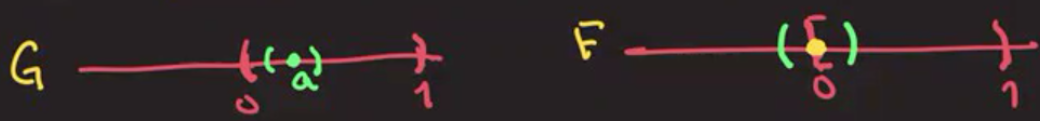
\includegraphics[scale=0.4]{images/2/1}
\end{center}
\end{ejemplo}

\begin{ejemplo}
	\begin{enumerate}
		\item $G=\{(x,y)\in\mathbb{R}^2\ni x^2+y^2<1\}$ es abierto. 
		\item $F=\{(x,y)\in \mathbb{R}^2\ni x^2+y^2\leq 1\}$ no es abierto. 
	\end{enumerate}
\begin{center}
	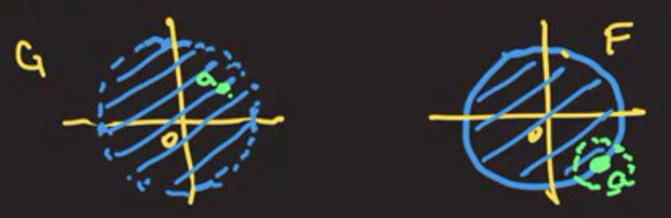
\includegraphics[scale=0.4]{images/2/2}
\end{center}
\end{ejemplo}

\begin{ejemplo}
	\begin{enumerate}
		\item $G=\{(x,y)\in\mathbb{R}^2\ni 0<x<1, y=0\}$ no es abierto de $\mathbb{R}^2$. 
		\item $F=\{(x,y)\in \mathbb{R}^2\ni 0<x<1\}$ es abierto de $\mathbb{R}^2$. 
	\end{enumerate}
	\begin{center}
		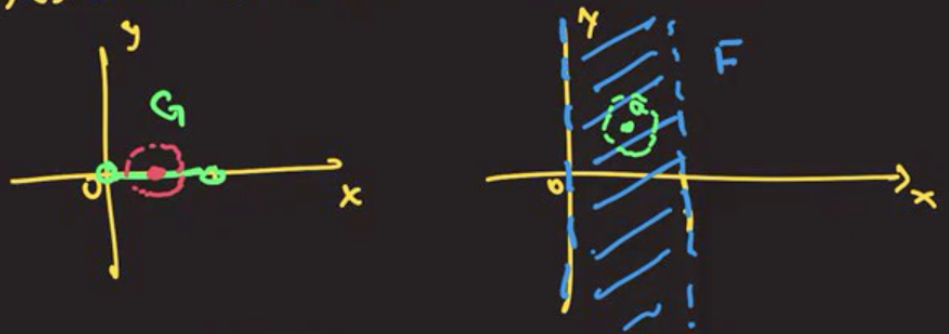
\includegraphics[scale=0.4]{images/2/3}
	\end{center}
\end{ejemplo}
\begin{ejemplo}
	$\Phi$ es abierto.
\end{ejemplo}

\begin{prop}
	Una bola abierta es abierto. 
\end{prop}
\begin{proof}
	Sea $x\in B_r(a)$ y considere la bola centrada en $x$ y de radio $r-d(a,x)$. A probar: $B_{r-d(a,x)}(x)\subset B_r(a)$. Sea $y\in B_{r-d(a,x)}(x)$. Entonces, 
	\begin{align*}
		d(a,y) &\leq d(a,x)+d(x,y)\\
		&< d(a,x)+[r-d(a,x)]\\
		&= r
	\end{align*}
$\implies y \in B_r(a)$. 

 	\begin{center}
 	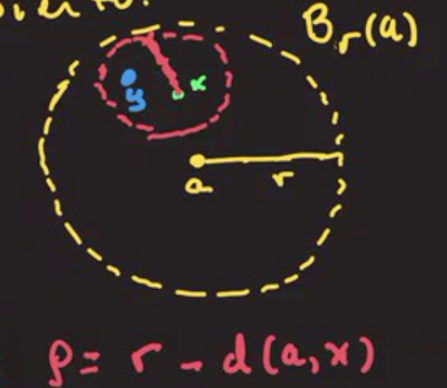
\includegraphics[scale=0.4]{images/2/4}
 \end{center}
\end{proof}

\begin{teorema}
	Considere $(\mathbb{R}^n,d)$: 
	\begin{enumerate}
		\item $\Phi$ y $\mathbb{R}^n$ son abiertos. 
		\item La intersección de dos abiertos de $\mathbb{R}^n$ es abierto de $\mathbb{R}^n$. 
		\begin{cajita}
			Por inducción, se deduce que la intersección finita de abiertos es abierto. 
		\end{cajita}
		\item La unión de cualquier colección de abiertos es un abierto de $\mathbb{R}^n$. 
	\end{enumerate}
\end{teorema}

\begin{proof}
	\begin{enumerate}
	\item OK. 
	\item Sea $A$ y $B$ abiertos de $\mathbb{R}^n$. A probar: $A\cap B$ es abierto. Sea $x\in A\cap B$, entonces: 
	\begin{enumerate}
		\item $x\in A$, abierto, $\implies \ \exists r>0\ni d(x,z)<r$, para $z\in A$. 
		\item $x\in B$, abierto, $\implies \ \exists r'>0\ni d(x,w)<r$, para $w\in B$.  
	\end{enumerate}
	\begin{center}
	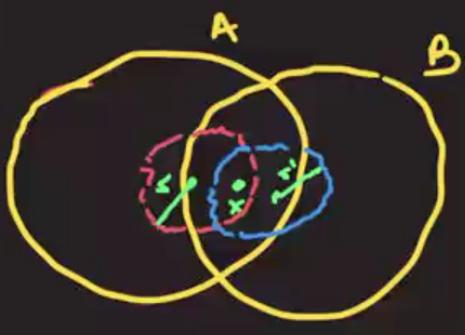
\includegraphics[scale=0.4]{images/2/5}
\end{center}
	$\implies$ Hagamos $r=\min\{r,r'\}\implies $ si $y\in \mathbb{R}\ni d(x,y)<r\implies y\in A$ y $y\in B\implies y\in A\cap B\implies A\cap B$ es abierto en $\mathbb{R}^n$. 
	
	\item Sea $\{G_\alpha\}$ una colección cualquiera de abierto de $\mathbb{R}^n$, y sea $G=\cup_{\alpha} G_\alpha$. Si $x\in G\implies x\in G_\lambda$, para algún $\lambda$. Como $G_\lambda$ es abierto $\implies \ \exists r>0 \ni B_r(x)\subset G_\lambda \subset \cup_\alpha G_\alpha =G$. 
		\end{enumerate}
\end{proof}

\begin{nota}
	La intersección de una colección infinita de abierto no necesariamente es abierto. En efecto considere: 
	\begin{align*}
		A_n &= \{x\in\mathbb{R}\ni -\frac{1}{n}<x<1+\frac{1}{n}\}, \quad n\in\mathbb{Z}^+\\
		A_1 &= (-1,2)\\
		A_2 &= \left(-\frac{1}{2}, \frac{3}{2}\right)\\
		&\vdots\\
		\implies A &= \cap_{n=1}^\infty A_n\\
	&= [0,1]\quad \text{¿Por qué cerrado?}
		\end{align*}
	
	\begin{cajita}
		Los $A_n$ son abiertos (por se bolas abiertas de $\mathbb{R}$)
	\end{cajita}
\end{nota}

\begin{definicion}
	Un subconjunto $\mathbb{F}$ en el métrico $(M,d)$ es cerrado si $\mathbb{F}^c$ es abierto. 
\end{definicion}
\begin{center}
	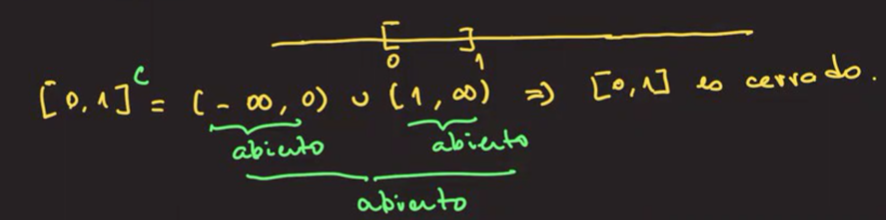
\includegraphics[scale=0.4]{images/2/6}
\end{center}

\begin{cajita}
	\begin{enumerate}
		\item Abierto: bola abierta contenida en $A$ es cada punto. 
		\begin{center}
			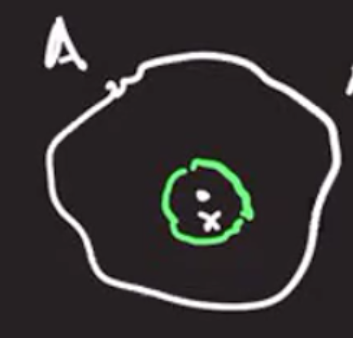
\includegraphics[scale=0.3]{images/2/7}
		\end{center}
	\item Topología (colección de todos los abiertos) en el métrico. 
	\item $F$ es cerrado si $F^c$ es abierto. 
	\item Abierto y cerrado no son negación uno del otro. \begin{enumerate}
		\item $\Phi$, $\mathbb{R}^n$ son abiertos y cerrados. 
		\item $[0,1)$ no es abierto ni cerrado. 
	\end{enumerate}
	\end{enumerate}
\end{cajita}

\begin{definicion}
	Sea $x\in M$ (espacio métrico), entonces cualquier conjunto que contiene un abierto $A\ni x\in A$ es una vecindad de $x$. 
\end{definicion}

\begin{ejemplo}
	Sea
	\begin{center}
		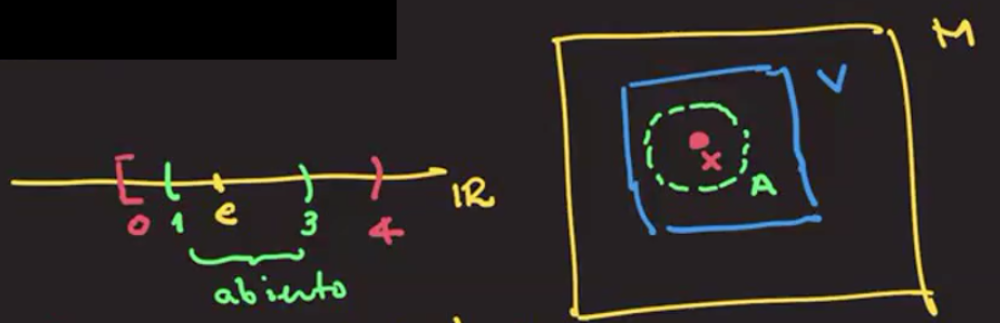
\includegraphics[scale=0.4]{images/2/8}
	\end{center}
\begin{enumerate}
	\item $[0,4)$ es na vecindad de $e$. 
	\item $(1,3)$ es vecindad abierta de $e$. 
	\item $\mathbb{R}$ es vecindad de $e$. 
	\item $(e-\varepsilon, e+\varepsilon)$ es vecindad de $e, \ \forall \varepsilon >0$. 
\end{enumerate}
\end{ejemplo}

\begin{definicion}
	Un punto $x\in M$ es punto interior de un conjunto $A\subseteq M$, si $A$ es una vecindad de $M$. 
	\begin{enumerate}
		\item $[0,1]$, $x=0$ y $x=1$; no son puntos interiores. El resto de punto $(0,1)$ son puntos interiores de $[0,1]$. 
		\item En $I=(0,1)$, todos son puntos interiores. 
		\item $\mathbb{R}\cap \mathbb{Z}\subseteq \mathbb{R}$. 
		\begin{center}
			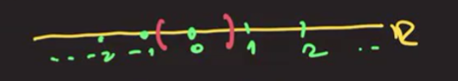
\includegraphics[scale=0.4]{images/2/9}
		\end{center}
	$\implies \mathbb{R}\cap \mathbb{Z}$ no tiene puntos interiores.  
	\end{enumerate}
\end{definicion}

\begin{definicion}
	Un punto $x$ es un punto de acumulación (o punto límite) de un conjunto $A\subseteq M$, si cada vecindad de $x$ contiene al menos un punto de $A$ diferente de $x$. Es decir, si 
	$$(B_r(x)-\{x\})\cap A\neq \emptyset, \quad \forall r>0.$$
\end{definicion}

\begin{ejemplo}
	$A=\{1,1/2,1/3,\cdots, 1/n, \cdots \}\subseteq \mathbb{R}\implies x=0$ es un punto de acumulación de $A$. 
	\begin{center}
		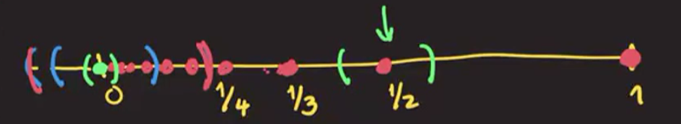
\includegraphics[scale=0.4]{images/2/10}
	\end{center}
\end{ejemplo}
	\begin{center}
	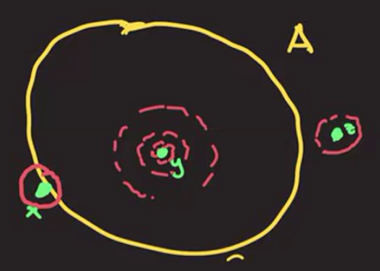
\includegraphics[scale=0.4]{images/2/11}
\end{center}

\begin{definicion}
	El conjunto de todos los puntos interiores de $A$ se llama interior de $A$ (Notación: $A^\circ$ o $int(A)$). 
	\begin{center}
		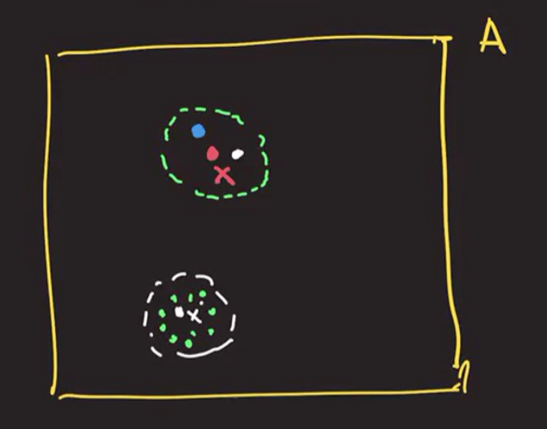
\includegraphics[scale=0.4]{images/2/12}
	\end{center}
	Es decir: 
	$$int(A)=\bigcup_{U\subset A, \  U \text{ es abierto.}} U$$
	i.e $int(A)$ en el abierto más grande contenido. 
	\begin{ejemplo}
		\begin{enumerate}
			\item $int[0,1]=(0,1)$. 
			\item $int \mathbb{R}\cap \mathbb{Z}=\emptyset$. 
			\item $int\mathbb{R}^n=\mathbb{R}^n$.
			\item $A$ es abierto $\iff A=int(A)$. 
		\end{enumerate}
	\end{ejemplo}
\end{definicion}

\begin{ejemplo}
	La cerradura de $A$ es el conjunto: 
	$$\overline{A}:= \bigcap_{A\subset F, \ \text{$F$ cerrado}} F $$
	\begin{nota}
		\begin{enumerate}
			\item $\overline{A}$ es cerrado. 
			\item $\overline{A}$ es el cerrado más pequeño que contiene a $A$. 
			\item $A$ es cerrado $\iff A=\overline{A}$. 
			\item Si $F$ es un cerrado que contiene a $A\implies A\subset \overline{A}\subset F$. 
		\end{enumerate}
	\end{nota}
\end{ejemplo}

\begin{definicion}
	La frontera de $A$ (denotada $bd(A)$ o $\partial A$), se define $$\partial A := \overline{A}-int(A).$$
	\begin{ejemplo}
		Sea $I=[0,1]\implies \overline{I}=[0,1]\implies int(I)=(0,1)\implies \partial A = \overline{I}-int(A)=\{0,1\}$. 
	\end{ejemplo}
\end{definicion}

\begin{definicion}
	El conjunto de todos los puntos de acumulación de un conjunto $A$ se llama conjunto derivada de $A$. Notación: $A'$. 
\end{definicion}

\begin{prop}
 Si $A\subset B\implies A'\subset B'$. \begin{proof}
			Sea $x\in A'$ (i.e $x$ es un punto de acumulación de $A$) $\implies \ \forall $ abierto $G\ni x\in G$, se tiene que 
			$$(G-\{x\})\cap A\neq \emptyset.$$
			Como $A\subset B\implies (G-\{x\})\cap A\subset (G-\{x\})\cap B\implies \emptyset \neq (G-\{x\})\cap A\subset A \subset (G-\{x\})\cap B\implies (G-\{x\})\cap B\neq \emptyset, \forall G\ni x\in G\implies x\in B'$. 
		\end{proof}
\end{prop}

\begin{prop}
	 $(A\cup B)'=A'\cup B'$
	 \begin{proof}Tenemos:
	 	\begin{enumerate} 
	 	\item[$(\supseteq)$] Sabemos que 
	 	\begin{enumerate}
	 		\item $A\subset A\cup B\implies A'\subset (A\cup B)'$.
	 		\item $B\subset A\cup B\implies B'\subset (A\cup B)'$. 
	 	\end{enumerate}
 	$\implies A'\cup B'\subset (A\cup B)'$. 
	 	\item[$(\subseteq)$] A probar: $A'\cup B'\subset (A\cup B)'$.
	 	\begin{cajita}
	 		\begin{enumerate}
	 			\item $\iff$ Si $x\in(A\cup B)'\implies x\in A'\cup B'$. 
	 			\item $\iff$ Si $x\not\in A'\cup B'\implies x\not\in (A\cup B)'$. 
	 		\end{enumerate}
	 	\end{cajita}
 	Sea $x\not\in A'\cup B' \implies x\not\in A'$ y $x\not\in B'$. $\implies$ Como $x\not \in A'\implies \exists G$, $\underbrace{abierto}_{x\in G}$, tal que $G\cap A\subset \{x\}$\footnote{$G\cap A=\emptyset$ o \xcancel{$G\cap A=\{x\}$}}.
 	\begin{center}
 		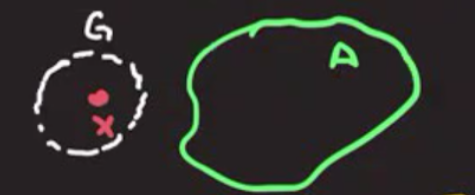
\includegraphics[scale=0.4]{images/2/13}
 	\end{center}
 Como $x\not\in B'\implies \exists H, \underbrace{abierto}_{x\in H}$, tal que $H\cap A\subset \{x\}$. Nótese que $G\cap H$ es abierto. Entonces, $x\in G\cap H$, y 
 $$(G\cap H)\cap (A\cup B)=(G\cap H\cap B)\subset \{x\}\cup \{x\}=\{x\}$$
 $\implies x\not\in (A\cup B)'\implies$ Si $x\not\in A'\cup B'\implies x\in (A\cup B')\implies (A\cup B)'\subset A'\cup B'\implies (A\cup B)'=A'\cup B'$. 
	 	\end{enumerate}
	 \end{proof}
\end{prop}

\begin{prop}
	$A$ es cerrado $\iff A'\subset A$.
	\begin{cajita}
		Un conjunto es cerrado $\iff$ contiene a sus puntos de acumulación.
	\end{cajita}
	\begin{proof}
		Se tiene: 
		\begin{enumerate}
			\item[$(\implies)$] \footnote{A probar: \begin{enumerate}
					\item $A'\subset A\iff$ si $x\in A'\implies x\in A$
					\item $A'\subset A\iff$ si $x\not\in A\implies x\not\in A'$. 
			\end{enumerate}}
		Sea $A$ cerrado y sea $p\not\in A\implies p\in A^c$, pero $A^c$ es un abierto $\ni p\in A^c$ y $A\cap A^c=\emptyset\implies p\not\in A'\implies A'\subset A$.
		\item[$(\impliedby)$] A probar: $A'\subset A\implies A$ es $\underbrace{cerrado}_{A^c\text{ es abierto}}$. Suponga que $A'\subset A$ y sea $p\in A^c$. $\implies p\not \in A'\implies \exists G$, abierto, tal que: $p\in G$ y $$(G-\{p\})\cap A=\emptyset.$$
		Como $p\not\in A\implies G\cap A=\emptyset \implies G\subset A^c$. Entonces, si $p\in A^c\exists$ abierto $G\ni p\in  G\subset A^c\implies A^c$ es abierto. $\implies A$ es cerrado. 
		\end{enumerate}
	\end{proof} 
\end{prop}

\begin{prop}
	Si $F$ es un superconjunto cerrdo de cualquier conjunto $A$, entonces $A'\subset F$. 
	\begin{proof}
		Sabemos que $F$ es cerrado y $A\subset F$. Como $A\subset F \implies A'\subset F\implies A'\subset F'$. Como $F$ es cerrado, entonces $F'\subset F\implies A'\subset F$. 
	\end{proof}
\end{prop}

\begin{prop}
	$A\cup A'$ es cerrado. 
\end{prop}

\begin{prop}
	$\overline{A}=A\cup A'$. 
	\begin{proof}
		\begin{enumerate}
			\item[$(\supseteq)$] Sabemos que $A\subset \overline{A}$. Por otra parte, $\implies A'\subset (\underbrace{\overline{A}}_{cerrado})'\subset \overline{A}\implies A'\subset \overline{A}\implies A\cup A'\subset \overline{A}$. 
			\item[$(\subseteq)$] A probar: $\overline{A}\subset A\cup A'$. Entonces, $A\subset \underbrace{A\cup A'}_{cerrado}\implies A\subset \overline{A}\subset A\cup A'$. 
			\begin{cajita}
				$$\overline{A}=\bigcap u\qquad \text{$u$ cerrado $\ni u\supset A$}$$
			\end{cajita}
		\end{enumerate}
	\end{proof}
\end{prop}

\begin{prop}
	Si $A\subset B\implies \overline{A}\subset \overline{B}$. 
	\begin{proof}
		Si $A\subset B\implies A'\subset B'\implies A\cup A'\subset B\cup B'\implies \overline{A}\subset \overline{B}$. 
	\end{proof}
\end{prop}

\begin{prop}
	$\overline{A\cup B}=\overline{A}\cup \overline{B}$. 
	\begin{proof}
		Tenemos:
		\begin{enumerate}
			\item[$(\subseteq)$] A probar: $\overline{A\cup B}\subset \overline{A}\cup \overline{B}$. Sabemos: 
			$$\begin{cases}
				A\subset \overline{A}\\ B\subset \overline{B}\
			\end{cases}\implies A\cup B\subset \underbrace{\overline{A}\cup \overline{B}}_{cerrado}.$$
		$\implies A\cup B\subset \overline{A\cup B}\subset \overline{A}\cup \overline{B}$. 
		\item[$(\supseteq)$] 
		$$\begin{cases}
			A\subset A\cup B &\implies \overline{A}\subset \overline{A\cup B}\\
		B\subset A\cup B &\implies \overline{B}\subset \overline{A\cup B}		\end{cases}\implies \overline{A}\cup \overline{B}\subseteq \overline{A\cup B}$$
	$\implies \overline{A\cup B}=\overline{A}\cup \overline{B}$. 
		\end{enumerate}
	\end{proof}
\end{prop}

\subsection{Axiomas de Kuratowski}

Se propone construir una topología de cerrados a partir de $K_1-K_4$. 

\begin{enumerate}
	\item[$K_1$]; $\overline{\emptyset}=\emptyset$
	\item[$K_2$]; $A\subset \overline{A}$.
	\item[$K_3$]; $\overline{\overline{A}} =\overline{A}$. 
	\item[$K_4$]; $\overline{A\cup B}=\overline{A}\cup \overline{B}$
\end{enumerate}

	\begin{center}
	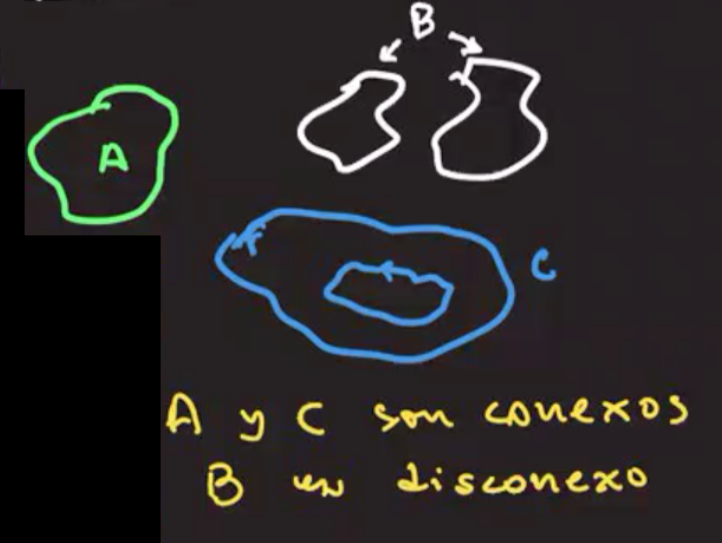
\includegraphics[scale=0.4]{images/2/14}
\end{center}

\subsection{Conjuntos conexos}

\begin{definicion}
	Un subconjunto $H$ del espacio métrico $M$ es disconexo, si existen abiertos $A$ y $B$ $\ni A\cap H\neq \emptyset, B\cap H\neq \emptyset, (A\cap H)\cap (B\cap H)=\emptyset$ y $(A\cap H)\cup (B\cap H)=H$. 
\end{definicion}

	\begin{center}
	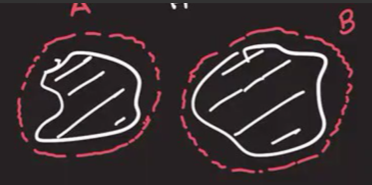
\includegraphics[scale=0.4]{images/2/15}
\end{center}

\subsubsection{Resumen}

	\begin{center}
	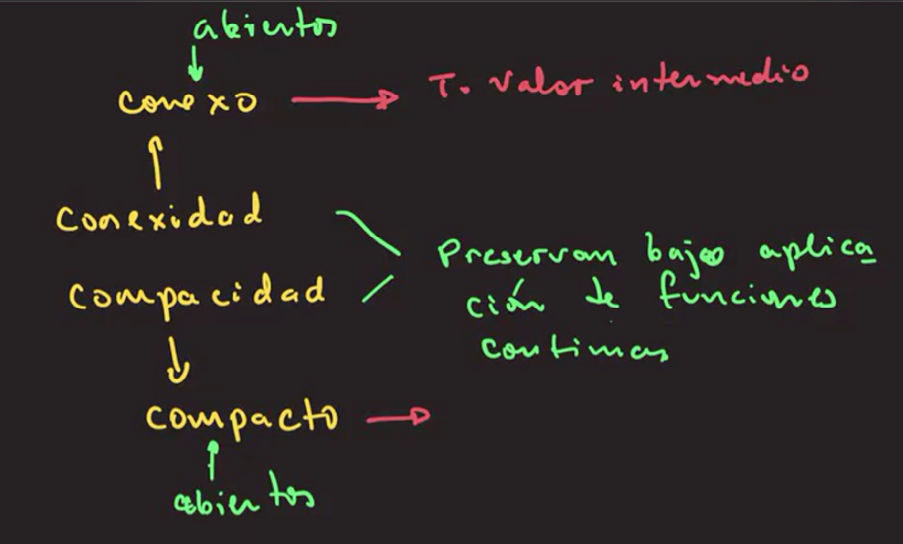
\includegraphics[scale=0.4]{images/2/16}
\end{center}

\begin{center}
	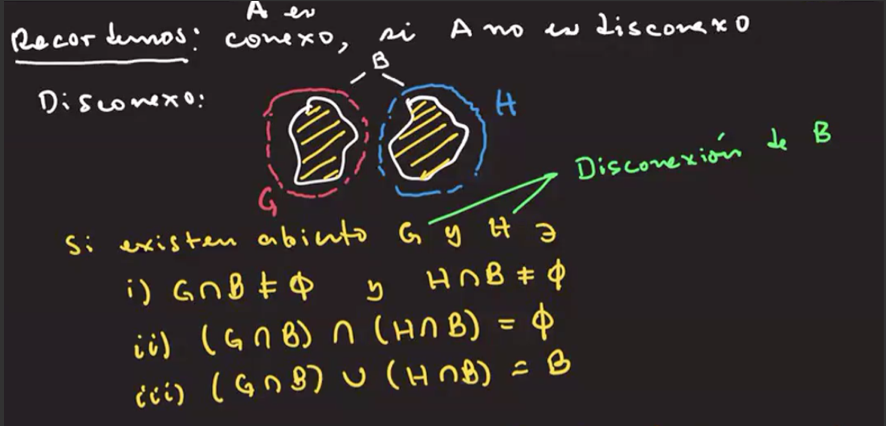
\includegraphics[scale=0.4]{images/2/17}
\end{center}

\begin{ejemplo}
	$\mathbb{Z}$ es disconexo en $\mathbb{R}$. En efecto, considere: $G=(-\infty, 1/2)$ y $H=(1/2,\infty)$. $\implies G$ y $H$ son una disconexión de $\mathbb{Z}\subseteq \mathbb{R}$. 
\end{ejemplo}
\begin{ejemplo}
	$\mathbb{Q}$ es disconexo en $\mathbb{R}$. En efecto, sea la disconexión: $G=(-\infty, \pi)$ y $H=(\pi, \infty)$.
\end{ejemplo}

\begin{teorema}
	$I=[0,1]$ es conexo en $\mathbb{R}$. 
	\begin{proof}
		Supóngase por el absurdo que $A$ y $B$ son una disconexión de $I$; i.e, $A\cap I$ y $B\cap I$ son no vacíos, disjuntos y su unión es $I$. 
		\begin{enumerate}
			\item Suponga que $1\in B$. 
			\begin{center}
				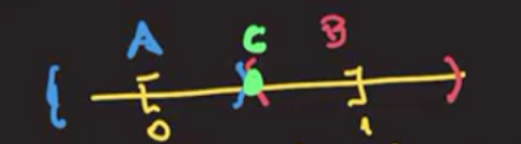
\includegraphics[scale=0.4]{images/2/18}
			\end{center}
			Como $I$ es acotado. $\implies A\cap I$ y $B\cap I$ también son acotados. Entonces, por el principio del supremo, $\exists c=\sup(A\cap I)>0$ y $c\in A\cup B$. 
			\item Si $c\in A$. $\implies c<1$. 
			\begin{center}
				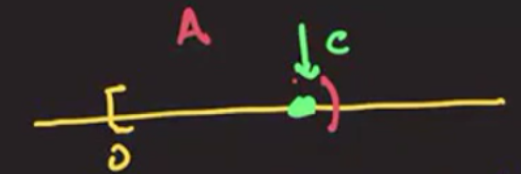
\includegraphics[scale=0.4]{images/2/19}
			\end{center}
	$\implies$ Como $A$ es abierto $\implies \exists B_r(c)\subset A\implies \exists \alpha \in A\ni c<\alpha$. $(\to\gets)\implies c\not\in A$. 
	\item Si $c\in B$. 
	\begin{center}
		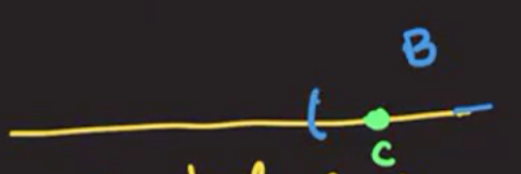
\includegraphics[scale=0.4]{images/2/20}
	\end{center}
	$\implies$ Como $B$ es abierto $\implies \exists c_1\in B\ni c_1<c$ y es tal que $[c_1,c]\cap (A\cap I)=\emptyset$ (i.e $c_1$ es una cota superior de $A\cap I$ y es menor que $c$)($\to\gets$). Entonces, que $c\in B$ ($\to\gets$). $\implies [0,1]$ es conexo.
		\end{enumerate}
	\end{proof}
\end{teorema}

\begin{corolario}
$(0,1)$ es conexo\footnote{Si $x$ es un intervalo. $\implies x$ es conexo.}. 
\end{corolario}

\begin{teorema}
	$\mathbb{R}^n$ es conexo.
	\begin{proof}
		Supóngase, por el absurdo, que $A$ y $B$ son una disconexión de $\mathbb{R}^n$. 
		\begin{center}
			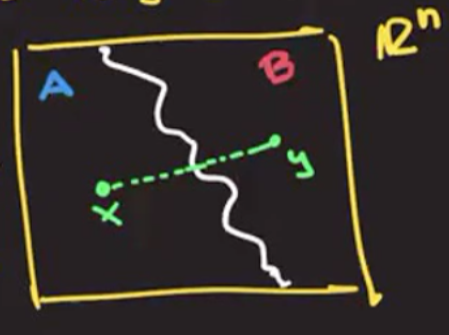
\includegraphics[scale=0.4]{images/2/21}
		\end{center}
		Sean $x\in A$ y $y\in B$, y considere el segmento de recta que une $x$ con $y$: 
		$$S=\{(1-t)x+ty:t\in[0,1]\}$$
		Sean: 
		\begin{align*}
			A_1 &= \{t\in \underbrace{\mathbb{R}}_{[0,1]}\ni (1-t)x+ty\in A\}\\
			B_1 &= \{t\in \underbrace{\mathbb{R}}_{[0,1]}\ni (1-t)x+ty\in B\}
		\end{align*}
	$\implies A_1\cap B_1 =\emptyset (\to\gets)$, ya que $A_1,B_1$ serían una disconexión de $[0,1]$. Entonces, $\mathbb{R}^n$ es conexo. 
	\end{proof}
\end{teorema}

\begin{teorema}
	Los únicos conjuntos abiertos y cerrados de $\mathbb{R}^n$ son $\emptyset$ y $\mathbb{R}^n$. 
	\begin{proof}
		Supóngase, por el absurdo, que $A\subset \mathbb{R}^n$, $A\neq \emptyset$ y $A\neq \mathbb{R}^n$, es abierto y cerrado de $\mathbb{R}^n$. Como $A$ es cerrado $\implies A^c=B$ es abierto. $\implies A\neq \emptyset, A\cap B=\emptyset$ y $A\cup B=\mathbb{R}^n$. $\implies A$ y $B$ forman una disconexión de $\mathbf{R}^n$ ($\to\gets$). $\implies$ Los únicos abiertos y cerrados de $\mathbf{R}^n$ son $\emptyset$ y $\mathbb{R}^n$. 
	\end{proof}
\end{teorema}

\begin{teorema}
	Un subconjunto de $\mathbb{R}$ es conexo $\iff$ es un intervalo.
	\begin{proof}Tenemos
		\begin{enumerate}
			\item[$(\impliedby)$] A probar: cada intervalo de $\mathbb{R}$ es un conexo. (Ver prueba de: $[0,1]$ es conexo). 
			\item[$(\implies)$] Sea $C\subseteq \mathbb{R}$ conexo. A probar: $C$ es un intervalo. Sean $a,b\in C\ni a<b$ y sea $x\in\mathbb{R}\ni a<x<b$. A probar: $x\in C$. Si $x\not\in C\implies (-\infty,x)$ y $(x,\infty)$ forman una disconexión de $c$. ($\to\gets$). $\implies x\in C\implies C$ es intervalo.  
		\end{enumerate}
	\end{proof} 
\end{teorema}

\subsection{Compactos}

Sea $A$ un subconjunto del espacio métrico $M$. Decimos que la familia de abierto $\{G_i\}_{i\in I}$ de $M$ es una cubierta abierta de $A$, si 
$$A\subseteq \bigcup_{i\in I}G_i$$

\begin{center}
	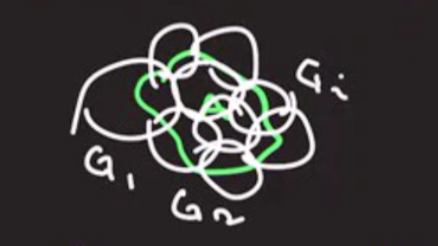
\includegraphics[scale=0.4]{images/2/22}
\end{center}

\begin{nota}
	En el caso de $M$, la cubierta abierta debe cumplir: 
	$$M=\bigcup_{i\in I}G_i$$
\end{nota}

\begin{definicion}
	Un subconjunto $A$ del espacio métrico $M$ es compacto si cada abierta de $A$ tiene subcubierta finita\footnote{Sigue cubriendo al conjunto $A$}. 
\end{definicion}

\begin{ejemplo}
	Sea $k=\{x_1,\cdots, x_n\}$ un subconjunto finito de $\mathbb{R}^n$ y sea $G=\{G_i\}_{i\in I}$ una cubierta abierta de $k$ (i.e $\bigcup_{i\in I}G_i \supseteq k$). Dado que $k$ es finito, basta un número finito de los $G_i$ para cubrir a $k$. $\implies$ es compacto. 
	\begin{center}
		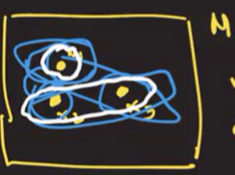
\includegraphics[scale=0.6]{images/2/23}
	\end{center}
\end{ejemplo}

\begin{ejemplo}
	Sea $H=[0,\infty)\subseteq \mathbb{R}$ no es compacto. En efecto, sea $G_n=(-1,n), n\in\mathbb{Z}^+$. 
	\begin{center}
		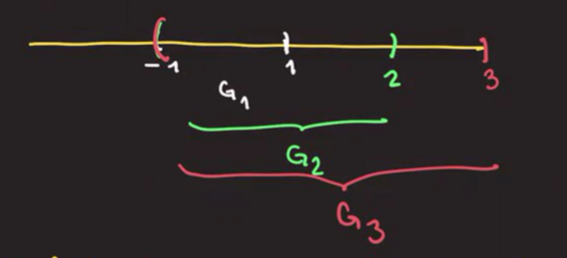
\includegraphics[scale=0.4]{images/2/24}
	\end{center}
$\implies G=\{G_n\}$ es una cubierta abierta de $H$. Suponga que $\{G_{n_1},G_{n_2},\cdots, G_{n_k}\}$ es una subcolección de $G$. Sea $M=\max\{n_1,n_2,\cdots, n_k\}$. $\implies G_{n_i}\subseteq G_M$, $i=1,\cdots, k \implies G_M=\bigcup_{i=1}^k  G_{n_i}$, pero, en particupar, $M\not\in \bigcup_{i=1}^k G_{n_i}\implies \{G_{n_1}, \cdots, G_{n_k}\}$ no cubre a $H$. Entonces, $G$ no tiene subcubierta finita para $H$. $\implies H$ no es compacto. 
\end{ejemplo}

\begin{ejemplo}
	Sea $H=(0,1)\subseteq \mathbb{R}$ y considere: 
	$$G_n=\left(\frac{1}{n}, 1-\frac{1}{n}\right), \quad n>2.$$
	\begin{center}
		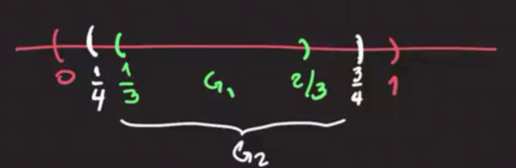
\includegraphics[scale=0.4]{images/2/25}
	\end{center}
$\implies G=\{G_n\}$ es una cubierta abierta de $H$, pero $G$ no tiene subcubierta finita para $H$. $\implies H$ no es compacto. 
\end{ejemplo}

\begin{prop}
	Sea $F$ un cubconjunto cerrado de un espacio métrico $M$. Entonces, $F$ es compacto. 
	\begin{center}
		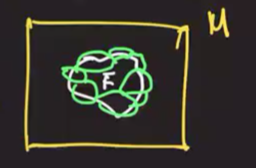
\includegraphics[scale=0.6]{images/2/26}
	\end{center}
\begin{proof}
	Sea $G=\{G_i\}$ una cubiera abierta de $F$. Como $F^c$ es abierto $\implies \left(\bigcup_{i\in I}G_i\right)\cup F^c$ es cubierta abierta de $M$, i.e. $\left(\bigcup_{i\in I}G_i\right)\cup F^c=M$. $\cdots $ es compacto, existe una subcubierta finita $M$, $\{G_{i_1}, G_{i_2},\cdots, G_{i_n},F^c\}$, tal que: $$G_{i_1}\cup G_{i_2}\cup \cdots\cup G_{i_n}\cup F^c=M$$

$\implies \{G_{i_1}, \cdots, G_{i_n}\}$ es una subcubierta finita para $F$. $\implies$ es compacto. \end{proof}
\end{prop}

\begin{teorema}[Heine-Borel]
	Un subconjunto $S$ de $\mathbb{R}^n$ es compacto $\iff$ es cerrado y acotado. 
\end{teorema}

\begin{ejemplo} Ejemplos.
	\begin{enumerate}
		\item $(0,1)$ no es compacto, ya que no es cerrado. 
		\item $[0,1]$ es compacto, por Heine-Borel.
	\end{enumerate}
\end{ejemplo}

\begin{cajita}
	\begin{enumerate}
		\item Si $S\subseteq \mathbb{R}$, compacto, $\implies S$ es cerrado y acotado. 
		\item Si $S\subseteq \mathbb{R}$ es cerrado y acotado. $\implies S$ es secuencialmente compacto $\implies S$ es compacto. \item Producto de una colección de conjuntos compacto. \textbf{(Teorema de Tíkonov -Tychonoff-)}
	\end{enumerate}
\end{cajita}

\begin{nota}
	Un espacio métrico $M$ es de Lindelof si cada cubierta abierta de $M$ tiene una subcubierta contable. 
\end{nota}

\begin{teorema}
	Si $S\subseteq \mathbb{R}$ es compacto, entonces $S$ es cerrado y acotado. 
	\begin{proof}
		A probar: $S$ es acotado. Considere, para $m\in \mathbf{Z}^+$, $H_m=(-m,m)$. Como cada $H_m$ es abierto y $S\subseteq \bigcup_{i=1}^\infty H_m=\mathbb{R}\implies \{H_m:m\in\mathbb{Z}^+\}$ es cubierta abierta de $S$. Como $S$ es compacto $\implies$ Hay una subcubierta finita $\{H_{m_1},\cdots, H_{m_n}\}$ para $S$, i.e. $S\subseteq \bigcup_{i=1}^n H_{m_n}=H_m=(-M,M)\implies M$ es acotado. \newline 
		
		A probar: $S$ es cerrado. $\iff S^c$ es abierto. Sea $u\in S^c$ y considere:
	$$G_n=\{y\in\mathbb{R}: |y-u|>1/n\, \quad n\in \mathbb{R}$$
	\begin{center}
	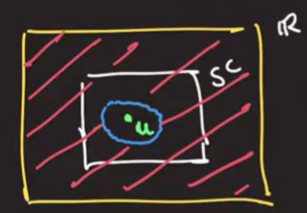
\includegraphics[scale=0.6]{images/2/27}
\end{center}
Note que los $G_n$ son abiertos y $\bigcup_{n=1}^\infty =\mathbb{R}-\{u\}$. Como $u\not\in S\implies S\subseteq \bigcup_{n=1}^{\infty} G_n\implies \{G_n\}$ es una cubierta abierta de $S$. Como $S$ es compacto. $\implies \exists m\in \mathbb{Z}^+\ni S\subseteq \bigcup_{n=1}^m G_n=G_m=\left[u-\frac{1}{m}, u+\frac{1}{m}\right]^c\implies S\cap \left(u-\frac{1}{m}, u+\frac{1}{m}\right)=\emptyset\implies \left(u-\frac{1}{m}, u+\frac{1}{m}\subset S^c\right)\implies S^c$ es abierto. $\implies S$ es cerrado. 
	\end{proof}
\end{teorema}

\begin{cajita}{Verificar.}
	¿Por qué Heine-Borel no aplica en un espacio métrico cualquiera? ¿Se cumple alguna de las implicaciones?
\end{cajita}

\begin{teorema}[Heine-Borel] El jefe mayor
	\begin{enumerate}
		\item Si $A\subseteq \mathbb{R}$ es compacto $\implies A$ es cerrado y acotado. 
		\item Si $A\subseteq \mathbb{R}$ es cerrado y acotado $\implies A$ es compacto. 
		\item Teorema de Tikonov. Producto cualquiera de compactos es compacto. 
	\end{enumerate}
\end{teorema}

\subsection{Hoja de repaso y parcial}

Reales y topología. 

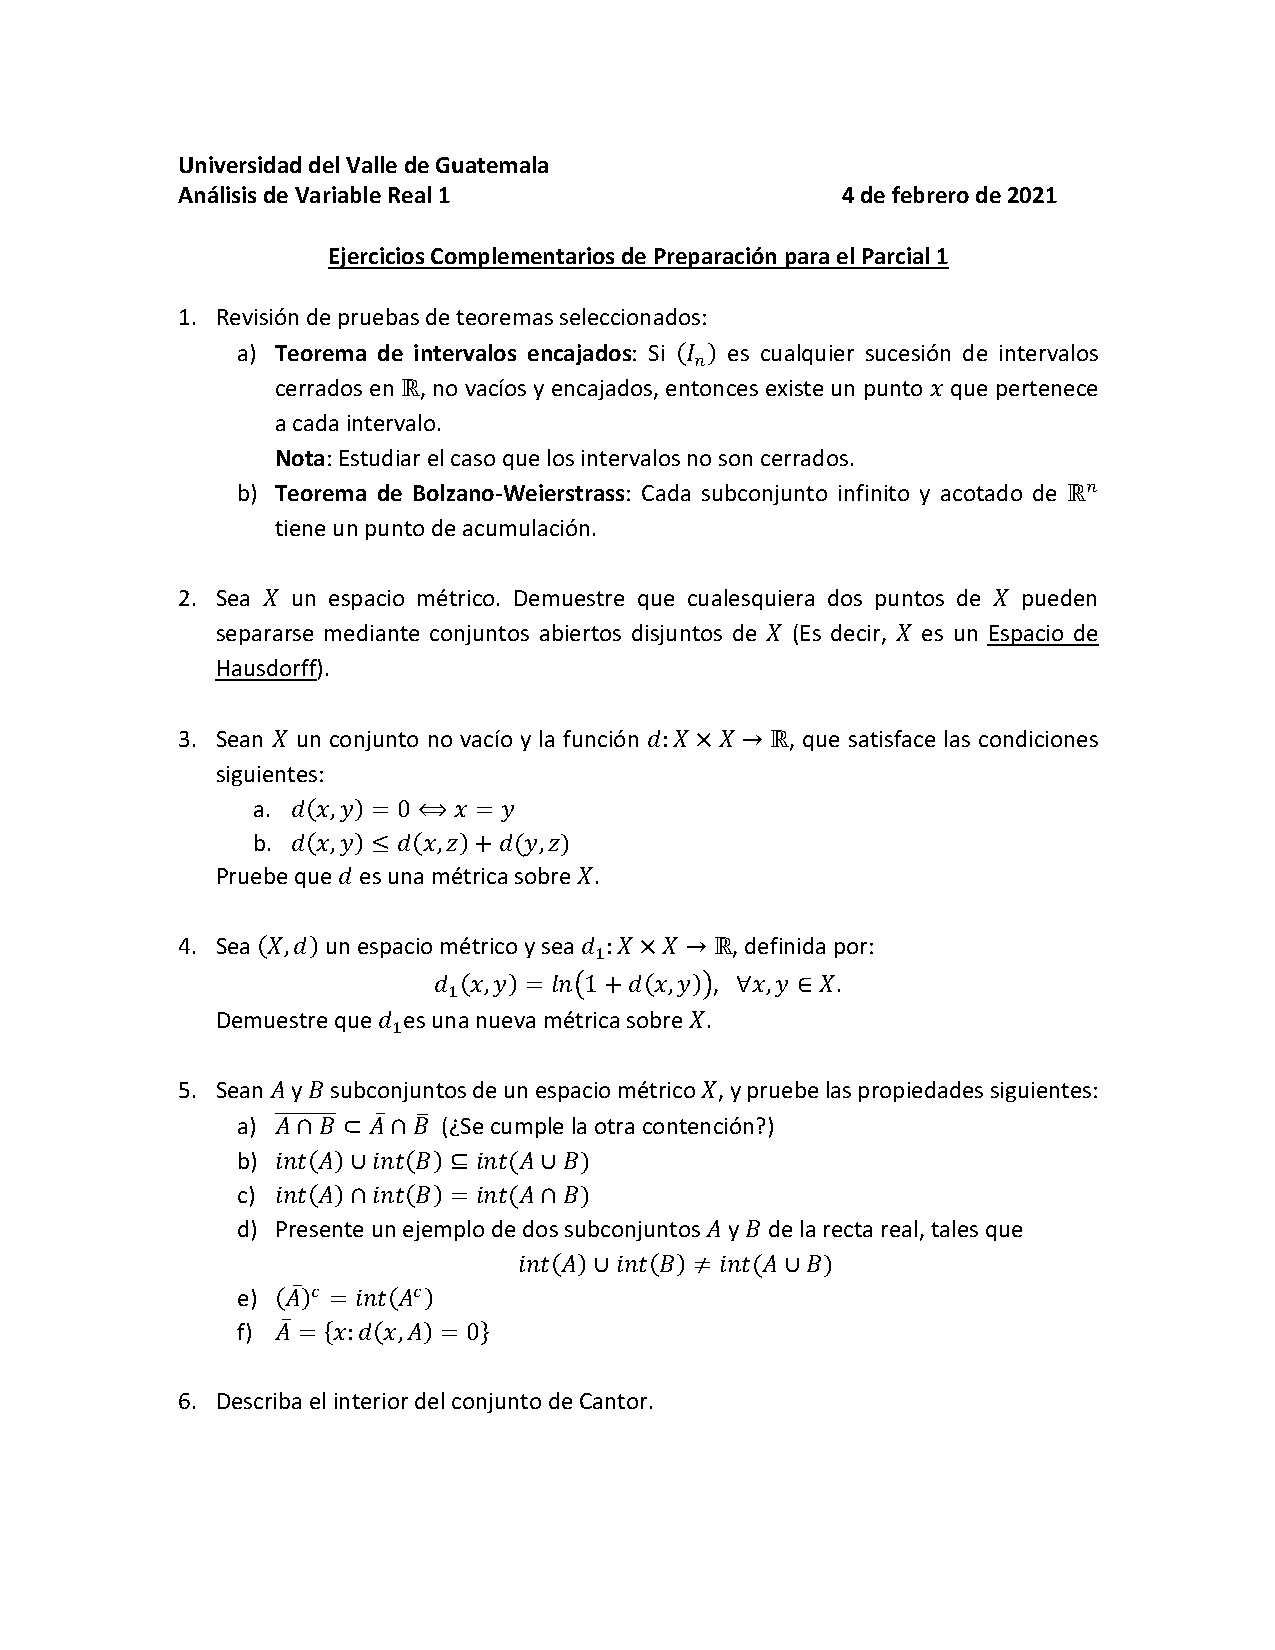
\includepdf[pages=-]{Apendices/Repaso1.pdf}
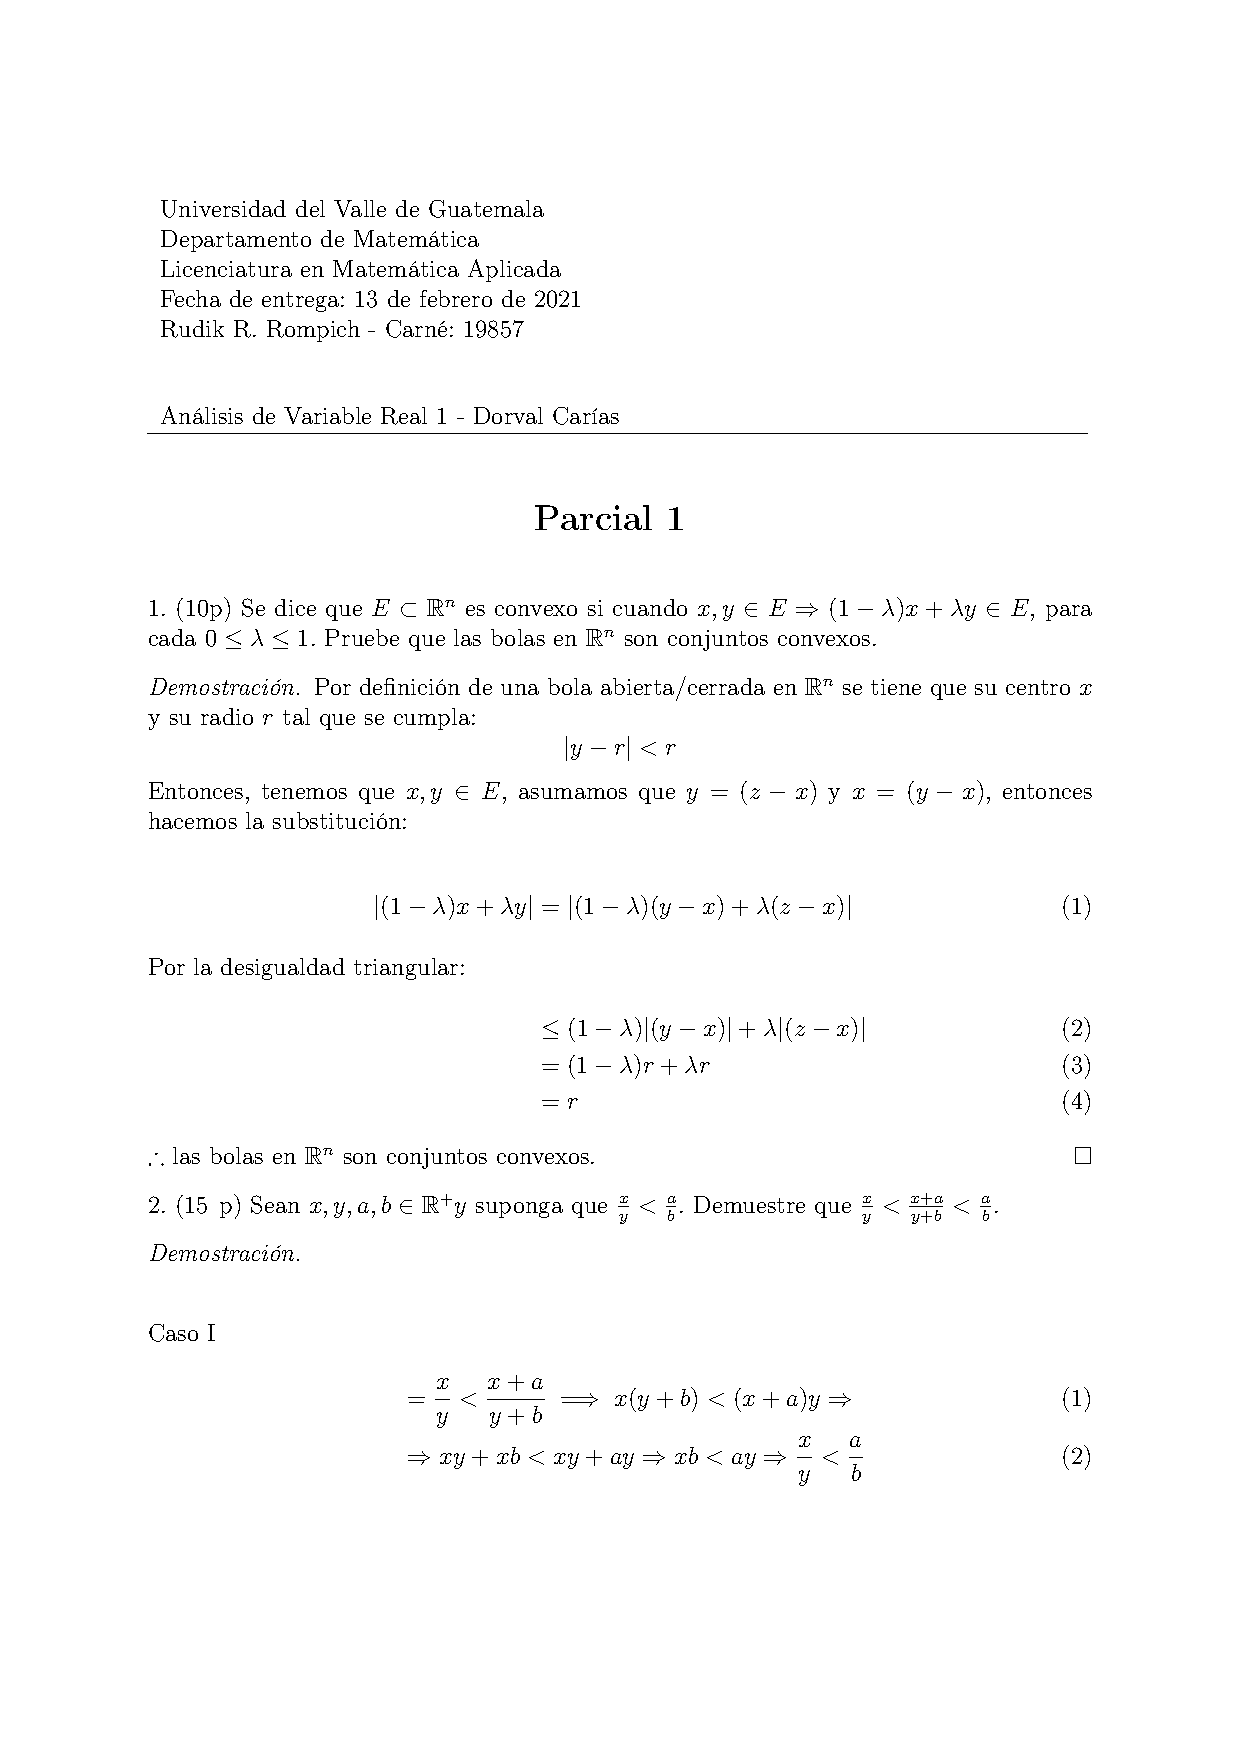
\includepdf[pages=-]{Apendices/Parcial1.pdf}

\subsubsection{Soluciones}

\begin{center}
	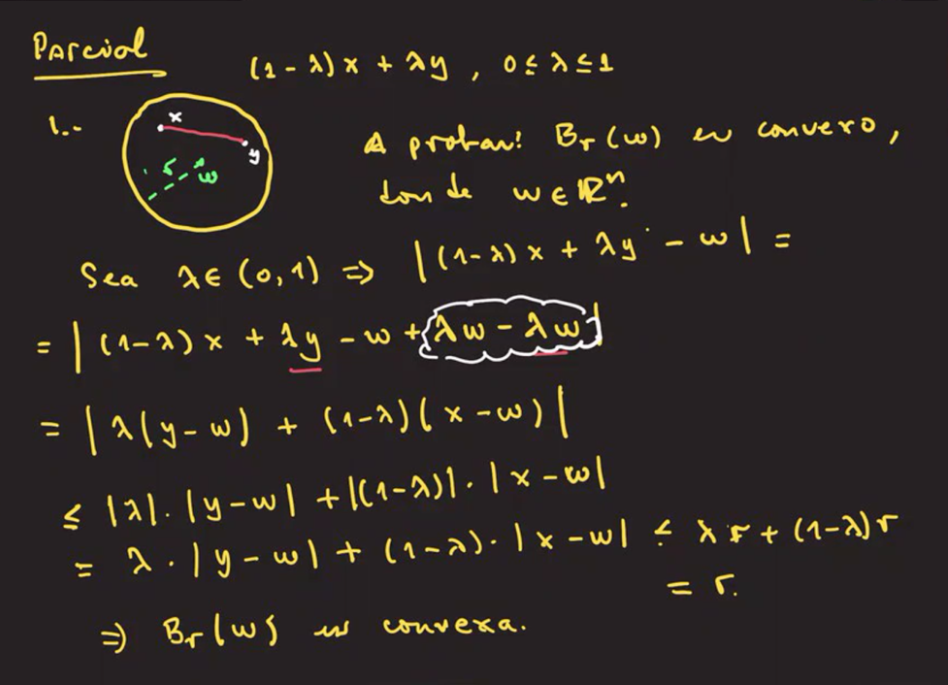
\includegraphics[scale=0.45]{images/2/28}
\end{center}
\begin{center}
	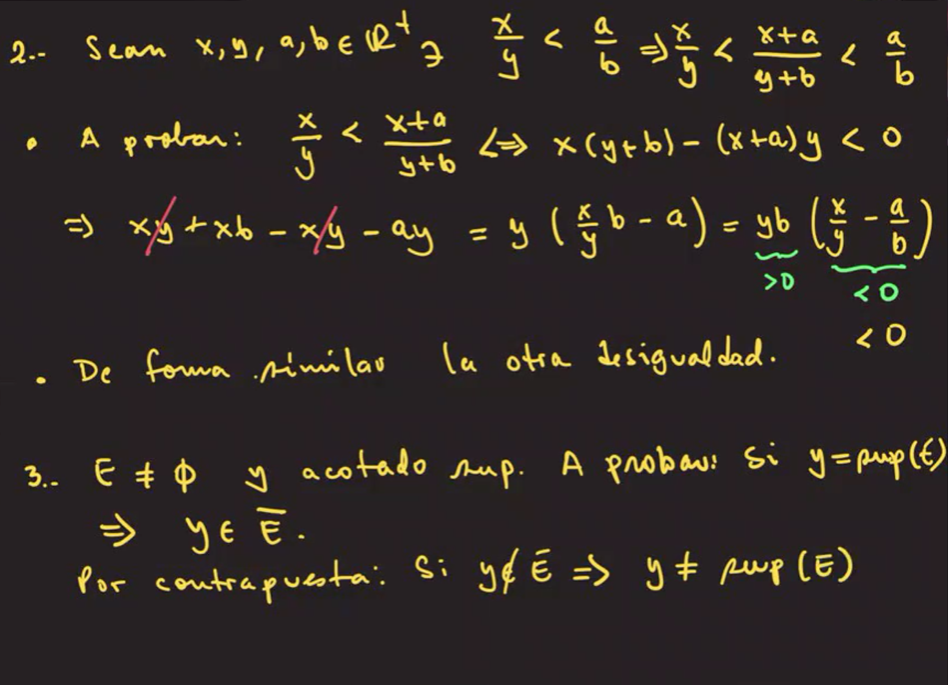
\includegraphics[scale=0.45]{images/2/29}
\end{center}
\begin{center}
	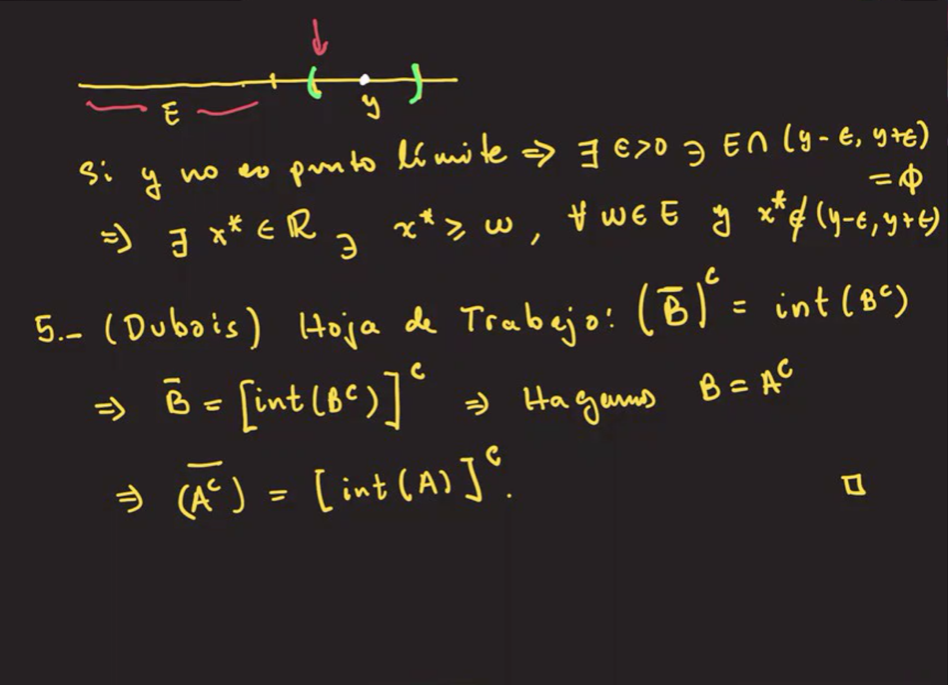
\includegraphics[scale=0.45]{images/2/30}
\end{center}

